% +--------------------------------------------------------------------+
% | Sample Chapter 3
% +--------------------------------------------------------------------+

\cleardoublepage

% +--------------------------------------------------------------------+
% | Replace "This is Chapter 3" below with the title of your chapter.
% | LaTeX will automatically number the chapters.
% +--------------------------------------------------------------------+
    %\renewcommand{\chaptername}{Part}
    %\renewcommand{\thechapter}{}
\chapter{Implementation}
\label{makereference}

\section{General overview of the system}
La cámara proporciona los pixeles de la imagen por bandas. Las primeras operaciones a realizar con estos datos son calcular la media, con ella la deviación y con esta la covarianza. Dadas la relativa simpleza de estas operaciones pero sus altos requisitos en memoria, estas tres operaciones son realizadas en una CPU y sus resultados enviados a la FPGA. La FPGA comenzará el cálculo de las operaciones posteriores solo cuando tenga los resultados completos de la covarianza.
Los datos calculados por la CPU son introducidos en la FPGA a través de FIFOs.
La FPGA calculará entonces la inversa de la matriz. Mientras tanto la CPU tendrá que escribir las medias calculadas y los valores que había recibido anteriormente de la cámara, uno por uno. Cuando termine la inversa, la FPGA realizará las dos últimas multiplicaciones de matrices y guardará los datos resultantes. Con el ultimo pixel procesado, la FPGA escribirá las anomalías ordenadas de mayor a menor en otra FIFO para ser leída por la CPU.

\pagebreak

\begin{figure}
\centering\textbf{
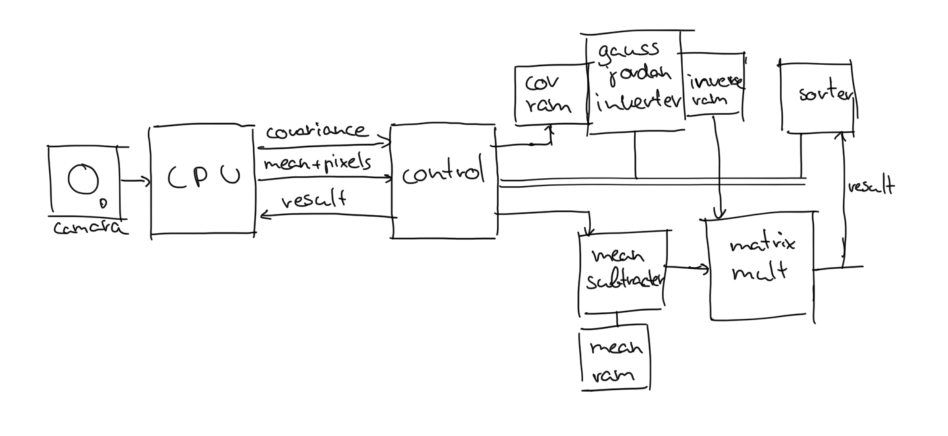
\includegraphics[height=7.5in]{figures/bus.png}}
\caption{A schematic of the whole system.}
  \label{fig:bus}
\end{figure}
\clearpage
\pagebreak

\section{Description by module}
\subsection{Control}
Este módulo actúa sobre los módulos inferiores, tanto para controlar el traspaso de datos entre ellos como para arbitrar el acceso a las RAMS y las FIFOs que comunican con la CPU.

Cabe mencionar que también realiza ciertas comprobaciones en la escritura de la covarianza para asegurar que la primera división de la inversa no se realiza con un 0, es decir, que la posición (0, 0) en la matriz de covarianzas es distinto de 0.
\\
\\
%\begin{lstlisting}
%IDLE:
%  if start then
%    goto READ
%
%READ:
%  while(fifo not empty)
%    read covariance row from fifo
%    if 0 then
%      swap
%    write covariance row to ram
%  if all rows written
%    goto INVERSE
%
%INVERSE:
%  start inverse
%  if inverse finished
%    goto MEAN SUBTRACTION
%
%MEAN SUBTRACTION:
%  start mean subtraction
%  if first result ready
%    goto MATRIX MULTIPLICATION
%
%MATRIX MULTIPLICATION:
%  start matrix multiplication
%  if first result ready
%    goto SORTER
%
%SORTER:
%  start SORTER
%  if matrix multiplication finished
%    write sorter results
%\end{lstlisting}
%
%
%\begin{figure}[h!]
%\centering
%\includegraphics[height=8in]{figures/flowchart.png}
%\caption{Tengo que elegir como lo prefiero}
%  \label{fig:ventana}
%\end{figure}
%\clearpage

\subsection{Inverter}
La inversa es el módulo más complejo y que más recursos hardware consume. Además, el estudio realizado en software ha mostrado que es con diferencia el paso más susceptible de empeorar la precisión de los resultados finales. Por estas razones se ha hecho especial hincapié en su diseño.

\begin{figure}[h!]
\centering\textbf{
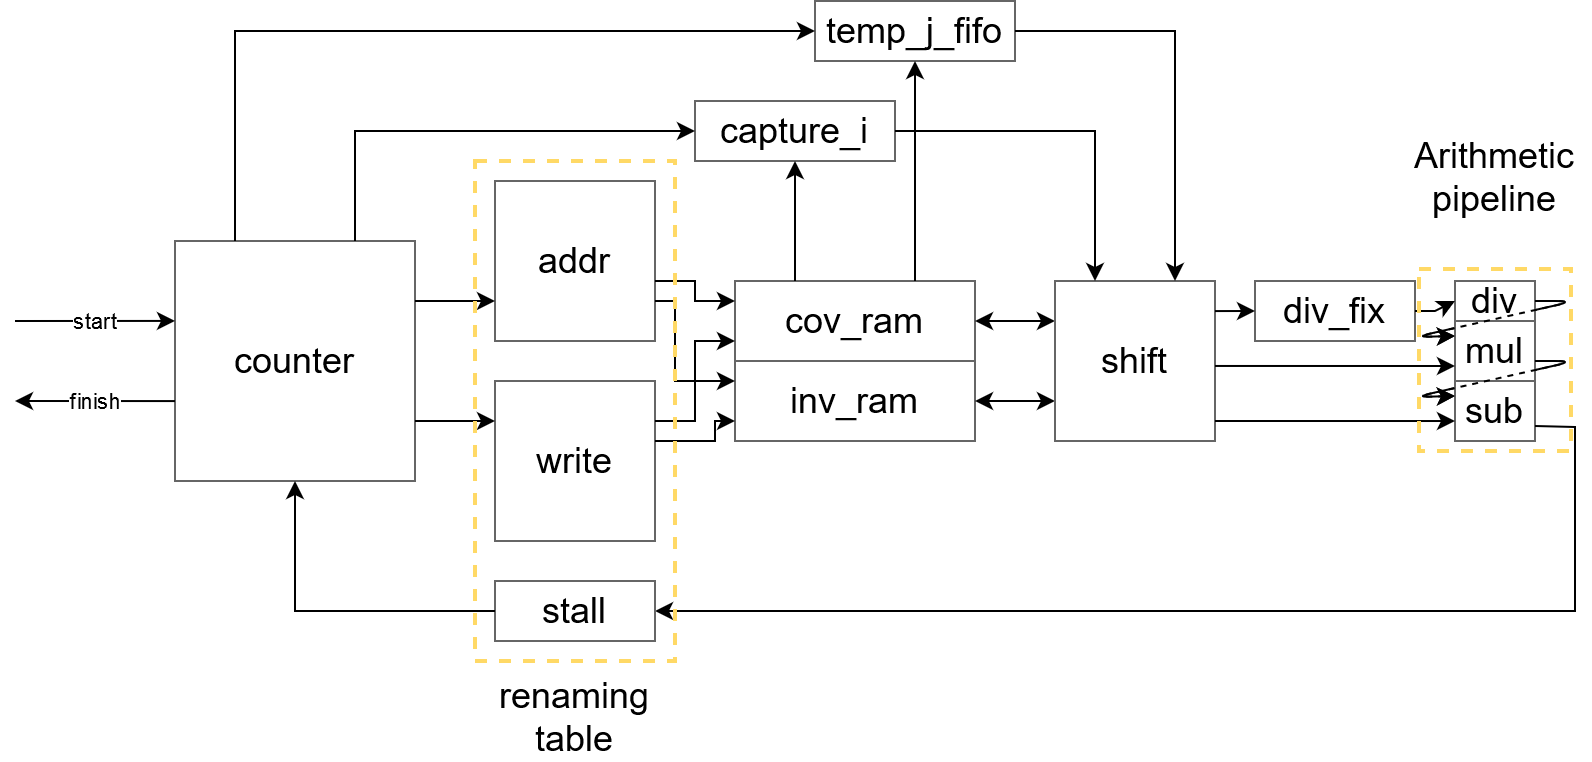
\includegraphics[height=2.5in]{figures/gauss.png}}
\caption{Schematic of the implemented inverter}
  \label{fig:gauss}
\end{figure}
Como se puede ver en \autoref{fig:gauss}, existen numerosos procesos y submódulos dentro del inversor. El proceso que actúa como interfaz al exterior es \textit{counter}, que como su nombre indica contiene contadores para calcular las filas que se deben leer, escribir, etc. Es el proceso principal del módulo. Los contadores son traducidos a direcciones por otro par de procesos, más concretamente \textit{addr}, \textit{write} y \textit{stall} y una tabla de renombrado a la que estos tres tienen acceso. Los datos que son leídos de las memorias pasan entonces a estar guardados en almacenamientos temporales o directamente a las unidades aritméticas. Antes de las unidades aritméticas se encuentra otro proceso, \textit{shift}, que desplaza los datos según se modeló en software. Estas unidades son usadas para los tres pasos del algoritmo -triangulo superior, inferior y diagonal- y es el proceso \textit{counter} el que controla este orden. El resto de procesos se explicarán más detalladamente dentro del capítulo.


\subsubsection{Optimizaciones del algoritmo de cara a hardware}
Para mejorar el rendimiento del módulo, las operaciones sobre la matriz $A$ y la matriz $A{-1}$ se ejecutan de forma simultánea. Además, se aprovecha el pipeline del divisor y de los DSP para encolar todas las operaciones consecutivas posibles. Solo ocurre una espera, concretamente mientras se estén procesando cálculos con la fila pivote actual.
La siguiente tabla muestra las unidades aritméticas que se encuentran dentro del módulo y sus latencias. Estas latencias representan la longitud de su pipeline.
\newcommand{\hr}[1]{%
  \colorbox{red!20}{$\displaystyle#1$}}
\newcommand{\hg}[1]{%
  \colorbox{green!20}{$\displaystyle#1$}}
\newcommand{\hb}[1]{%
  \colorbox{blue!20}{$\displaystyle#1$}}
\begin{center}
 \begin{tabular}{|c c c c|} 
 \hline
 Arithmetic Unit & Latency & Quantity & Remarks\\ [0.5ex] 
 \hline\hline
 \hr{Division} & 77 & 1 & Only one division is required each cycle \\ 
 \hline
 \hg{Multiplication} & 6 & bands*2 & To compute a whole row for both $A$ and $A^-1$ \\
 \hline
 \hb{Subtraction} & 2 & bands*2 & To compute a whole row for both $A$ and $A^-1$ \\
 \hline
\end{tabular}
\end{center}

Las siguientes ecuaciones indican que cálculos se encuentran en un momento dado dentro del pipeline de los DSP. Los resultados de cada operación son enviados directamente al cálculo de la siguiente operación, a la vez que los contadores controlan que los demás operandos lleguen en el momento correcto.
\newcommand{\twodots}{\MTFlushSpaceAbove\vdotswithin{\gets}&&\vdotswithin{\gets}\MTFlushSpaceBelow}
\begin{align*}
%A^{-1}[87]\gets&A^{-1}[87]-A[i]^{-1}*A[87][i]/A[i][i],\ 
%&A[87]\gets&A[87]-A[i]*A[\jv][i]/A[i][i]\\
%\twodots
A^{-1}[86]\gets&A^{-1}[86]-A[i]^{-1}*\hr{A[86][i]/A[i][i]},\ 
&A[86]\gets&A[86]-A[i]*A[86][i]/A[i][i]\\
\twodots
A^{-1}[10]\gets&A^{-1}[10]-A[i]^{-1}*\hr{A[10][i]/A[i][i]},\ 
&A[10]\gets&A[10]-A[i]*A[10][i]/A[i][i]\\
A^{-1}[9]\gets&A^{-1}[9]-\hg{A[i]^{-1}*div\_result},\ 
&A[9]\gets&A[9]-\hg{A[i]*div\_result}\\
\twodots
A^{-1}[3]\gets&A^{-1}[3]-\hg{A[i]^{-1}*div\_result},\ 
&A[3]\gets&A[3]-\hg{A[i]*div\_result}\\
A^{-1}[2]\gets&\hb{A^{-1}[2]-mul\_result},\ 
&A[2]\gets&\hb{A[2]-mul\_result}\\
A^{-1}[1]\gets&\hb{A^{-1}[1]-mul\_result},\ 
&A[1]\gets&\hb{A[1]-mul\_result}\\
A^{-1}[0]\gets&\hb{sub\_result},\ 
&A[0]\gets&\hb{sub\_result}
\end{align*}

Uno de los operandos es la fila \textit{j}, que es usada en dos momentos diferentes dentro del algoritmo. Puesto que no se puede realizar una segunda lectura de la BRAM ya que esta se encuentra ocupada realizando las lecturas de las próximas operaciones, este dato es guardado en el momento de lectura en una FIFO y será leído en el momento en el que se vuelva a necesitar.
\newcommand{\highlight}[1]{%
  \colorbox{yellow!20}{$\displaystyle#1$}}
\begin{figure}[h!]
\[A^{-1}[j] \gets \highlight{A^{-1}[j]}-A[i]*\highlight{A[j][i]}/A[i][i]\]
\caption{Como se puede observar en el algoritmo, la fila j es usada dos momentos diferentes.}
\end{figure}
\\
\\
Además, se puede observar que en el primer paso en el que se construye la matriz triangular superior, el algoritmo exige una comprobación en la fila pivote y un posible intercambio de filas. Esto es necesario ya que este valor es posteriormente el dividendo, por lo que un 0 provocaría un fallo en el cálculo.
\\
Las lecturas de memoria BRAM tienen un ciclo de latencia, por lo que leer un valor no adecuado dos ciclos seguidos -en el caso de leer un valor adecuado y uno no adecuado, existiría la posibilidad de realizar un trueque de filas inplace con el pivote y la fila justo posterior- no solo añadiría latencia al cálculo si no que incrementaría la complejidad del módulo. Por lo tanto las comprobaciones del dividendo se realizan en las escrituras, y los trueques necesarios se graban en una tabla de renombrado que será comprobada en el momento de la lectura. Esto permite asegurar que las lecturas van a ser siempre válidas para el cálculo. En el caso de la primera división, este dividendo viene directamente de la CPU y el módulo superior \textit{control} se encarga de reordenar esta fila si fuera necesario.
\\
Esta tabla de renombrado se encuentra en registros por lo que es posible acceder a ella sin ninguna latencia y al solo contener indices no sobrecarga los recursos de la FPGA. Además, esta tabla es local, por lo que los resultados tienen que ser reordenados en la propia RAM antes de salir del módulo de la inversa. Puesto que estos trueques solo ocurren en el cálculo del triangulo superior, se puede aprovechar el triangulo inferior para reordenarlos. El sistema de reordenamiento es muy simple, los datos entran en el pipeline según el orden que existe en la tabla de renombrado y son escritos en su orden natural. Esto implica que los resultados de este reordenamiento van a ser correctos siempre y cuando ambas filas que hayan rotado se encuentren en el pipeline de procesado, que en el caso de  punto fijo tiene aproximadamente un tamaño de 90. Resultados experimentales muestran que rara vez hay que rotar filas -aunque lo suficiente como para ser recomendable la inclusión de un método que lidie con ello-, y que rara vez estas rotaciones exceden más una o dos posiciones en adelante.
\\
\\
En la transformación a aritmética entera se descubrió que el cálculo de la inversa es que más error llega a introducir en los resultados finales del algoritmo, por lo tanto se ha hecho estudio exhaustivo en  sobre como minimizarlo. Para ello ha sido necesario reducir los valores en los que la precisión limitada producía desbordamientos y aumentar valores pequeños para otorgarles más peso en las operaciones. Además, al realizar las operaciones de generación de identidad, triangulo superior, inferior y diagonal de forma independiente, se ha podido colocar diferentes desplazamientos y afinar todavía más la resolución del algoritmo. Estas operaciones se encuentran en el proceso \textit{shift}.
\\
También cabe decir que existe un error en la generación de divisores de Xilinx. Cuando se introducen números cerca del limite de precision se pierde el control del signo. Por lo tanto se ha colocado un proceso, \textit{div\_fix}, antes de la división que convierte todos los operandos introducidos en positivos y guarda su posición en un pipeline. En el momento de producirse los resultados, se comprueba el tag en el pipeline, se calcula el negativo y se sustituye si es necesario.

\subsection{Mean subtract}

\begin{figure}[h!]
\centering\textbf{
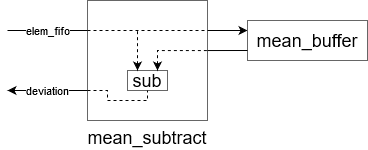
\includegraphics[height=1.5in]{figures/subtract.png}}
\caption{Schematic of mean subtract.}
  \label{fig:subtract}
\end{figure}
El módulo de \textit{mean subtract} recibe la media calculada y los pixeles originales de la imagen y los resta. Este cálculo es la deviación y aunque ya había sido calculada por la CPU, es posible que esta última deseche los datos para liberar espacio. El cálculo de la media si que se requiere puesto que se supone que al ser su tamaño mucho menor, la CPU pueda mantenerlo en memoria. En el caso de que la deviación pueda ser recibida directamente desde la CPU, este módulo puede ser simplemente borrado.
El módulo recibe los elementos desde el módulo superior que los lee de una misma FIFO. Los primeros elementos son la media y son guardados en una BRAM que es tratada como un buffer circular, y los elementos que le siguen son restados directamente y devueltos al módulo superior de nuevo.


\subsection{Matrix multiplication}


\newcommand\rb{\colorbox{red!20}}
\newcommand\bb{\colorbox{blue!20}}
\newcommand\gb{\colorbox{green!20}}
\newcommand\rr{\rowcolor{red!20}}
\newcommand\br{\rowcolor{blue!20}}
\newcommand\gr{\rowcolor{green!20}}
Como se denota arriba \ref{alternativa}, este cálculo puede ser implementado de dos maneras diferentes.
\noindent Following will be a comparison of the first required multiplication in both methods:
\begin{quote}
	\((x-\mu)^{T} K^{-1}_{N \times N}\):	
	A row from the inverse and the whole column of the deviation get read, each element multiplied with its correspondent and all products added together. If stalls were to be avoided, this sum would need to be computed every cycle, which can easily be achieved with an adder tree.
\end{quote}

\begin{figure}[h]%t=top, b=bottom, h=here
\[
\begin{pmatrix}
\rr a & b & c \\ 
\br d & e & f \\ 
\gr g & h & i
\end{pmatrix}
*
\begin{pmatrix}
1\\
2\\
3
\end{pmatrix}
=
\begin{pmatrix}
\rr 1*a+2*b+3*c\\
\br 1*d+2*e+3*f\\
\gr 1*g+2*h+3*i
\end{pmatrix} 
\]
\caption[Optional: Short caption to appear in List of Figures]{First proposed method for the computation of a single pixel: red, blue and green represent data processed in the first, second and third cycles respectively. Note that the entire deviation data of that pixel gets used every cycle}
\end{figure}
\pagebreak
		
\begin{quote}
	\(K^{-1}_{N \times N} (x-\mu)\):
	The inverse gets also read row by row, but the deviation matrix only by elements. Each element of the first row of the matrix gets multiplied with the first element of the deviation, the result accumulated, and continued with the next pair row/element. This goes for \(N\) cycles, that is, a whole inverse matrix and a whole pixel in the deviation matrix. The result is \(N\) accumulated values which get flushed every \(N\) cycles, which ends up being the same throughput as the former method.
\end{quote}

\begin{figure}[h]%t=top, b=bottom, h=here
\[
\begin{pmatrix}
\rb1 & \bb 2 & \gb 3
\end{pmatrix}
*
\begin{pmatrix}
\rr a & b & c \\ 
\br d & e & f \\ 
\gr g & h & i
\end{pmatrix}
=
\begin{pmatrix}
\rb{1*a}+\bb{2*d}+\gb{3*g} & \rb{1*b}+\bb{2*e}+\gb{3*h} & \rb{1*c}+\bb{2*f}+\gb{3*i}
\end{pmatrix} 
\]
\caption[Optional: Short caption to appear in List of Figures]{Second proposed method: red, blue and green represent data processed in the first, second and third cycles respectively. Here only an element of the deviation data gets accessed each cycle.}
\end{figure}

While both methods have equivalent cost in time -the former has the added latency of the adder tree, the latter the latency of the accumulators- and also similar cost in DSP usage, data input by row is less taxing on the CPU and its FIFO structure can be reused for the second multiplication. Henceforth, the second approach was chosen.

\pagebreak

\begin{figure}[h!]
\centering\textbf{
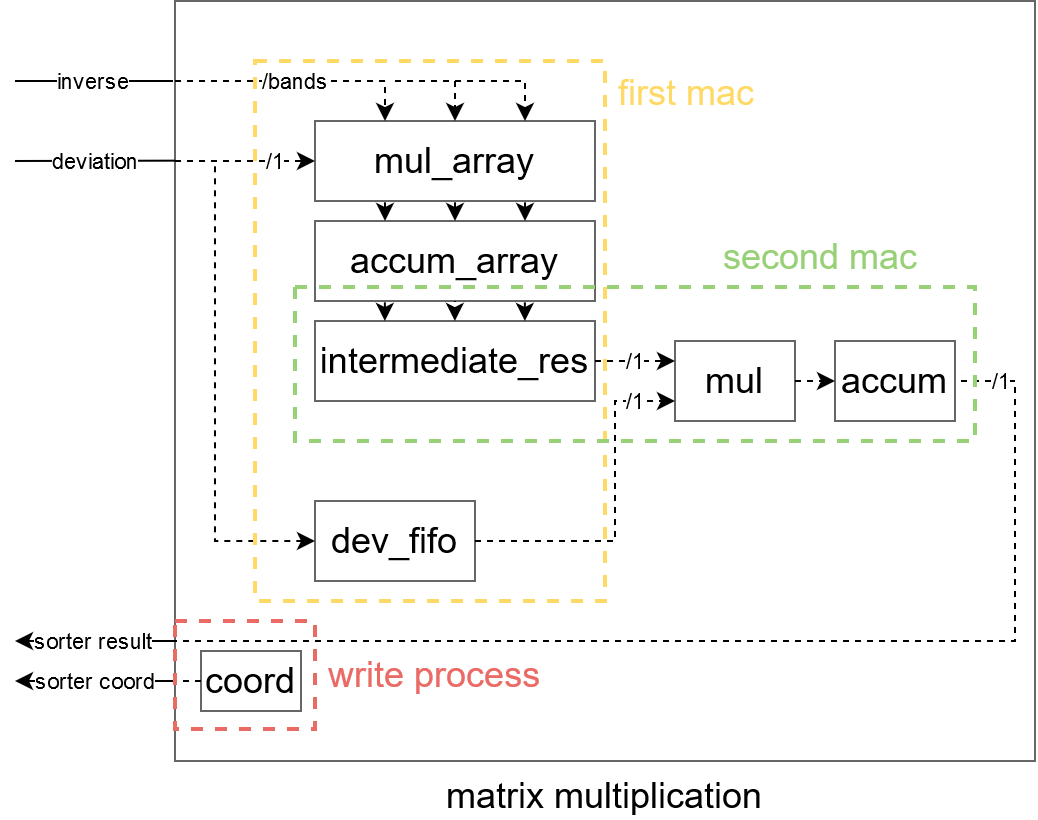
\includegraphics[height=3.5in]{figures/mult.png}}
\caption{Schematic of the dual matrix multiplier}
  \label{fig:mult}
\end{figure}

The second multiplication is similar in both steps, a \(1 \times N\) by \(N \times 1\) multiplication. One operand comes every cycle and each \(N\) cycles all products get added together. This sum is realized through an accumulator.\\

The module contains three subprocesses:
\begin{itemize}
	\item \emph{first\_mac} reads the inverse and performs its multiplication with the received deviation. This deviation is also stored in a FIFO. The products are then accumulated till a whole pixel has been computed.
	\item \emph{second\_mac} stores the results of \emph{first\_mac} in registers and performs the multiplication with data from the FIFO, with the result being accumulated. Every cycle, the registers are shifted so a new multiplication is done.
	\item \emph{write\_proc} controls the writing of the results from \emph{second\_mac} to the sorter and computes the coords.
\end{itemize}



\subsection{Coordinate sorter}
Este módulo recibe un valor y un par de coordenadas cada \textit{bandas} ciclos. Estos valores son escritos en una memoria BRAM que actúa como una lista ordenada. Cada valor introducido es comparado con la cabeza de la lista, el valor más alto guardado y el otro es guardado en una variable temporal y comparada con el segundo valor en la lista, así sucesivamente. Puesto que se recibe un valor cada \textit{bandas}, el numero máximo de valores posibles a almacenar en esta lista es también \textit{bandas}. El resto de valores son desechados. Cuando se ha introducido el ultimo valor, el módulo comunica los pixeles más altos, es decir, más anómalos, al módulo superior para que estos sean comunicados a la CPU.

\begin{figure}[h!]
\centering\textbf{
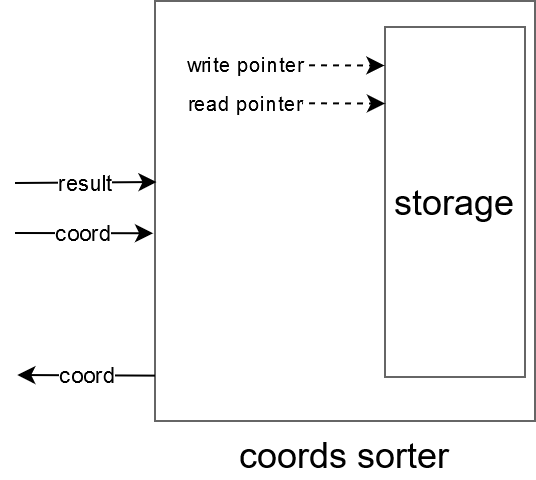
\includegraphics[height=2.5in]{figures/sort.png}}
\caption{Schematic of the coordinate sorter}
  \label{fig:sorter}
\end{figure}
